\section{Dominoes}

The objective is to find out where the complexity lies in the Tetris. To contribute something in this matter we will study Tetris with dominoes. From the above results it has been seen that adding more complexity in the set of pieces makes it more complicated.

Focusing on 2-\textsc{tris}, Tetris with dominoes, will help in our goal. As it can be seen in Table~\ref{tab:tt}, the variation 2-\textsc{tris-NoRotation} \clearing\ is in \npc and the only domino's problem closed. Let's start by defining the game.

\subsection{Definitions}

Before proceeding further, we first define how domino piece states are mapped onto the board and how the pieces move. A domino state \( \piece[\VD][\theta][i][j][f] \) is mapped into:

\begin{center}
\begin{equation}
\piece[\VD][\theta][i][j][f] \mapsto  \begin{cases}
    \{ \cell, \cell[i][j+1] \} &\text{if } \theta = 0^\circ\\
    \{ \cell, \cell[i-1][j] \} &\text{if } \theta = 90^\circ\\
    \{ \cell, \cell[i][j-1] \} &\text{if } \theta = 190^\circ\\
    \{ \cell, \cell[i+1][j] \} &\text{if } \theta = 270^\circ
\end{cases}
\end{equation}
\end{center}

The mapping works like a clock: the piece's position serves as the center, and the second cell acts as the clock's handle. Figure~\ref{dom:mapping} illustrates the mapping for all orientations.

\begin{figure}[h]
    \centering
    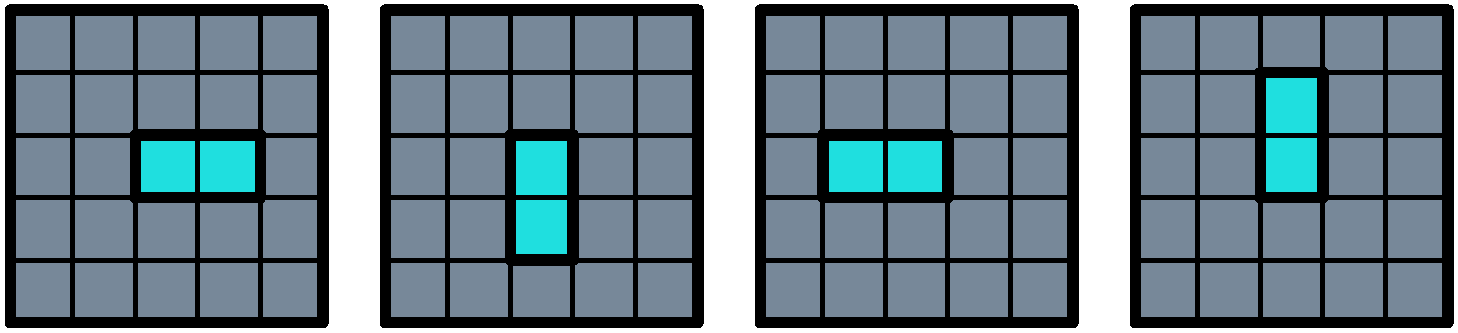
\includegraphics[width=0.6\textwidth]{./pictures/dominoes/mapping.pdf}
    \caption{The mapping of a piece placed at the center of the square. From left to right, the orientations are \(0^\circ\), \(90^\circ\), \(180^\circ\), and \(270^\circ\), respectively.}
    \label{dom:mapping} 
\end{figure}

The moves set has the standard drop and slides will be used. For the fix move the \emph{partial lock rule} will be used, witch only fixes pieces that are completely inside the board. Regarding rotation moves, most modern Tetris implementations employ the Super Rotation System (SRS), the official Tetris Guideline standard for tetromino rotation behavior \cite{SRS}. In SRS, when a piece is rotated and overlaps with filled cells, the system attempts to reposition the piece by testing a predefined set of translations. 

Following a similar approach, we define a Dominoes Rotation System (DRS), described in Table~\ref{dom:rotation}.


\begin{table}[ht]
\centering
\begin{tabular}{|c || c | c || c | c ||} 
 \hline
  & \multicolumn{2}{| c ||}{ $\VD$ } & \multicolumn{2}{| c ||}{$\HD$} \\
 \hline               
 & Test 1  & Test 2 & Test 1  & Test 2 \\ 
 \hline               
 $r_+$ & $\vcenter{\hbox{
\includegraphics[scale=0.3]{./pictures/dominoes/rotation/vert_clock_1.pdf}}}$ & $\vcenter{\hbox{
\includegraphics[scale=0.3]{./pictures/dominoes/rotation/vert_clock_2.pdf}}}$  & $\vcenter{\hbox{
\includegraphics[scale=0.3]{./pictures/dominoes/rotation/horit_clock_1.pdf}}}$  & $\vcenter{\hbox{
\includegraphics[scale=0.3]{./pictures/dominoes/rotation/horit_clock_2.pdf}}}$ \\ 
 \hline                             
 $r_-$ & $\vcenter{\hbox{
\includegraphics[scale=0.3]{./pictures/dominoes/rotation/vert_anti_1.pdf}}}$ & $\vcenter{\hbox{
\includegraphics[scale=0.3]{./pictures/dominoes/rotation/vert_anti_2.pdf}}}$  & $\vcenter{\hbox{
\includegraphics[scale=0.3]{./pictures/dominoes/rotation/horit_anti_1.pdf}}}$  & $\vcenter{\hbox{
\includegraphics[scale=0.3]{./pictures/dominoes/rotation/horit_anti_2.pdf}}}$ \\ 
 \hline
\end{tabular}
\caption{The DRS rotation table. The top rows indicate the initial orientation of the piece: vertical (\(\VD\)) or horizontal (\(\HD\)). The left columns specify the rotation direction (\(r_+\) for clockwise, \(r_-\) for counterclockwise), and the tests describe possible placements. In each image, the original piece is shown in white, while the resulting piece is displayed over it.}
\label{dom:rotation}
\end{table}

Intuitively, DRS tries to rotate a piece by moving it slightly: \(r_+\) attempts to place the piece to the right or above, while \(r_-\) shifts it to the left or below, depending on its orientation. When a piece is rotated, DRS performs the following steps:
\begin{enumerate}
    \item First, DRS attempts the rotation using Test 1. 
    \item If the resulting piece overlaps with a filled cell, DRS proceeds to Test 2. 
    \item If Test 2 also fails, the piece cannot be rotated, and the move is deemed illegal.
\end{enumerate}

Figure~\ref{dom:drs} provides an example of the DRS rotation system in action.

\begin{figure}[ht]
  \centering
  \begin{subfigure}[b]{0.15\textwidth}
    \centering
    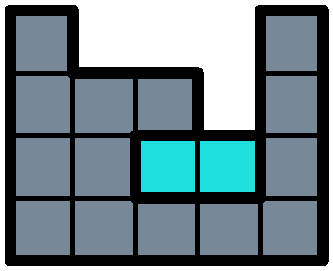
\includegraphics[width=0.9\textwidth]{pictures/dominoes/drs-1.pdf}
    \caption{}
  \end{subfigure}
  \begin{subfigure}[b]{0.15\textwidth}
    \centering
    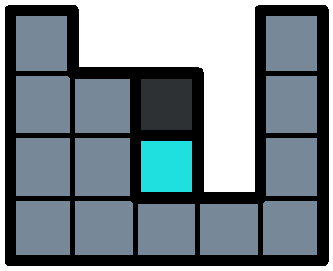
\includegraphics[width=0.9\textwidth]{pictures/dominoes/drs-2.pdf}
    \caption{}
  \end{subfigure}
  \begin{subfigure}[b]{0.15\textwidth}
    \centering
    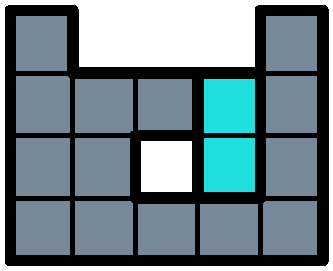
\includegraphics[width=0.9\textwidth]{pictures/dominoes/drs-3.pdf}
    \caption{}
  \end{subfigure}
  \caption{When rotating clockwise the domino in (a) DRS first ties to place it like (b), but this position isn't legal. Test 2 tries to place it in the right column which results a valid position.}
  \label{dom:drs}
\end{figure}

DRS allows pieces to move freely across the board, enabling not only standard movements but also upward motion in a staircase-like pattern, as shown in Figure~\ref{dom:staircase}. Most importantly, DRS makes it possible to place a domino in almost any position.

\begin{figure}
  \centering
  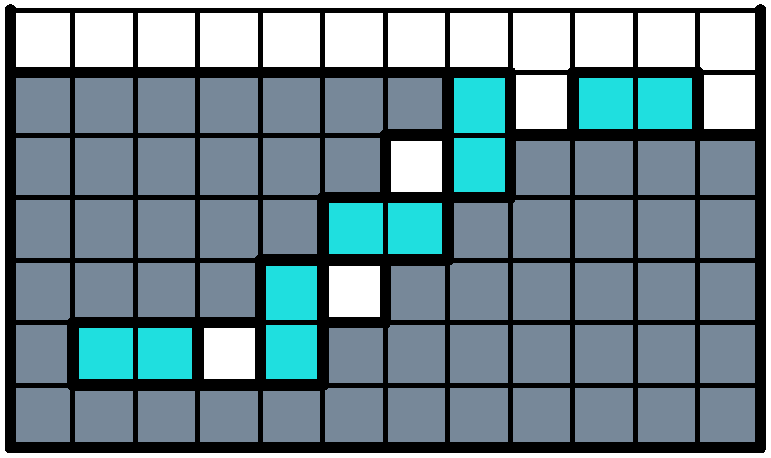
\includegraphics[width=0.3\textwidth]{pictures/dominoes/staricase.pdf}
  \caption{The overvevirew of a tragjectory starting at the left to the rightmost piece. The moves sequece is: $(3 \times s_r, 8 \times r_+, 2 \times s_r)$}
  \label{dom:staircase}
\end{figure}

\begin{definition}
  Given an $n \times m$ board $B$, a \emph{reachable path} is a sequence of adjacent cells \( p = (c_1, c_2, \dots, c_k) \) such that:
\begin{enumerate}
  \item  $c_1$ is in row $n$
  \item $c_l = \cell\) and \( c_{l+1} = \cell[i+1][j] \) implies \( c_{l+2} \neq \cell[i+2][j] \)
  \item $  c_l = \cell$, \( c_{l+1} = \cell[i+1][j] \) and \( c_{l+2} = \cell[i+1][j \pm 1] \) if cell $\cell[i][j \pm 1]$ of $B$ is filled respectively.
\end{enumerate}
\end{definition}

The four conditions ensure that the path starts from the top row, doesn't go vertically and the staircase pattern has its ladders.

\begin{lemma0} \label{lem:path}
For any board configuration \( B \), there exists a trajectory $\sigma$ that places a domino in any position in a reachable path. 
\end{lemma0}


\begin{proof}
  Let \( p = (c_1, c_2, \dots, c_k) \) be such a path. We assume that the domino is initially placed in cells \( c_1 \) and \( c_2 \) since the path start at the top of the board.

  We prove that, given a domino placed in \( c_l \) and \( c_{l+1} \), there exists a move or a combination of moves that places the domino in \( c_{l+1} \) and \( c_{l+2} \). By repeating this argument, the entire trajectory can be constructed.

  If \( c_l \), \( c_{l+1} \), and \( c_{l+2} \) are in the same row (or column) the domino is orientated vertically (horizontally) and can reach the3 next path cell with via a slide (drop). The remaining cases occur at turns. When the path passes through filled cells, there are eight possible scenarios, as shown in Figure~\ref{dom:turns}.

\begin{figure}[h]
  \centering
  \begin{subfigure}[b]{0.1\textwidth}
    \centering
    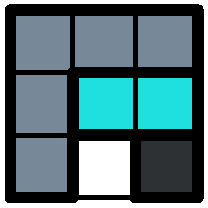
\includegraphics[width=0.9\textwidth]{pictures/dominoes/turns/turn_1.pdf}
    \caption{}
    \label{dom:turn1}
  \end{subfigure}
  \begin{subfigure}[b]{0.1\textwidth}
    \centering
    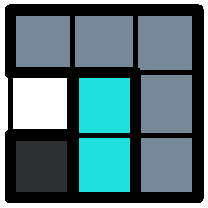
\includegraphics[width=0.9\textwidth]{pictures/dominoes/turns/turn_2.pdf}
    \caption{}
    \label{dom:turn2}
  \end{subfigure}
  \begin{subfigure}[b]{0.1\textwidth}
    \centering
    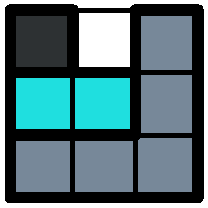
\includegraphics[width=0.9\textwidth]{pictures/dominoes/turns/turn_3.pdf}
    \caption{}
    \label{dom:turn3}
  \end{subfigure}
  \begin{subfigure}[b]{0.1\textwidth}
    \centering
    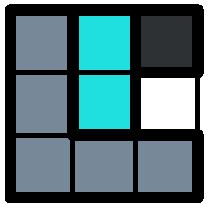
\includegraphics[width=0.9\textwidth]{pictures/dominoes/turns/turn_4.pdf}
    \caption{}
    \label{dom:turn4}
  \end{subfigure}
  \begin{subfigure}[b]{0.1\textwidth}
    \centering
    
\includegraphics[width=0.9\textwidth]{pictures/dominoes/turns/turn_5.pdf}
    \caption{}
    \label{dom:turn5}
  \end{subfigure}
  \begin{subfigure}[b]{0.1\textwidth}
    \centering
    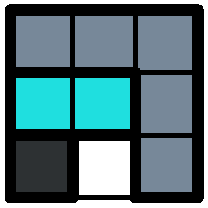
\includegraphics[width=0.9\textwidth]{pictures/dominoes/turns/turn_6.pdf}
    \caption{}
    \label{dom:turn6}
  \end{subfigure}
  \begin{subfigure}[b]{0.1\textwidth}
    \centering
    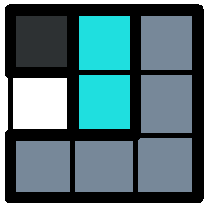
\includegraphics[width=0.9\textwidth]{pictures/dominoes/turns/turn_7.pdf}
    \caption{}
    \label{dom:turn7}
  \end{subfigure}
  \begin{subfigure}[b]{0.1\textwidth}
    \centering
    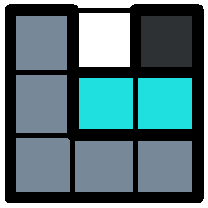
\includegraphics[width=0.9\textwidth]{pictures/dominoes/turns/turn_8.pdf}
    \caption{}
    \label{dom:turn8}
  \end{subfigure}
    \caption{The possible turns. The domino before the move is painted, and the destination cell is marked in white. In dark gray the corner cell that varies the moves to be done.} 
    \label{dom:turns} 
\end{figure}

The trajectory required to perform the move involves either one or two steps, depending on the state of the corner cell. The remaining cells can be in any configuration. Table~\ref{dom:turns-table} shows the necessary moves for each scenario based on whether the corner cell is filled.

\begin{table}[ht]
\centering
\begin{tabular}{|c || c | c | c | c | c | c | c | c |} 
 \hline
  & \ref{dom:turn1} & \ref{dom:turn2} & \ref{dom:turn3} & \ref{dom:turn4} & \ref{dom:turn5} & \ref{dom:turn6} & \ref{dom:turn7} & \ref{dom:turn8} \\
 \hline               
  filled & $ r_-  $ & $      r_-    $ & $   r_+, s_r  $ & $   r_+       $ & $   r_+       $ & $     r_-     $ & $   r_-       $ & $   r_+      $  \\
 \hline               
unfilled & $ r_-  $ & $     -       $ & $   r_+       $ & $   r_+       $ & $    -        $ & $  r_-, s_r   $ & $   r_-       $ & $   r_+      $  \\
 \hline               

\end{tabular}
\caption{The moves needed to do each turn of Table~\ref{dom:turns}.}
\label{dom:turns-table}
\end{table}

The path can be calculated in $\mathcal{O}(k)$.

\end{proof}


\subsection{Constructible Boards}

In this section, we present results on the structure of the initial constructible configurations that will subsequently be utilized to address each problem.

\begin{lemma0} \label{lem:floating}
  In any constructible board, for any filled cell $\cell$, the cells directly below it, $\cell[i-1][j-1]$, $\cell[i-1][j]$, and $\cell[i-1][j+1]$, cannot all be unfilled.
\end{lemma0}  

\begin{proof}  
Let \( B \) be an \( n \times m \) board containing such a filled cell $\cell$. Consider the sequence of boards \( B_0, B_1, \dots, B_k = B \), where \( B_0 \) is an empty board and \( B_k = B \). Assume, without loss of generality, that \( B_k \) is the first board in the sequence containing a filled cell \( c = \cell_k \) (the cell \( \cell \) in \( B_k \)) such that all the cells directly below it, $\cell[i-1][j-1]_k$, $\cell[i-1][j]_k$, and $\cell[i-1][j+1]_k$, are unfilled.  


The cell \( c \) cannot result from adding a domino that does not clear a row. Therefore, \( B_k \) must be obtained by adding a domino to \( B_{k-1} \) in such a way that it clears a row. Let \( r \) denote the row cleared in \( B_{k-1} \). In \( B_{k-1} \), clearing row \( r \) only modifies the cells below the ones in row \( r+1 \), so \( c \) must be in row \( r = i \). 

If the domino that clears the row also fills \( \cell[r+1][j]_{k-1} \), it implies that a vertically oriented domino has been placed in \( \cell[r+1][j]_{k-1} \) and \( \cell[r][j]_{k-1} \). Consequently, the cell \( \cell[r-1][j]_k \) would also be filled in order to fix the domino. Therefore, \( c \) originates from \( \cell[r+1][j]_{k-1} \) in \( B_{k-1} \).

If \( \cell[r][j]_{k-1} \) is filled, then one of \( \cell[r-1][j-1] \), \( \cell[r-1][j] \), and \( \cell[r-1][j+1] \) must be filled, since \( c \) is the first cell with this property. In that case, when row \( r \) is cleared, at least one cell below  must be filled. Therefore, \( \cell[r][j]_{k-1} \) must be unfilled.

Row \( r \) is cleared when the next piece is placed, so row \( r \) is fully filled except for \( \cell[r][j]_{k-1} \) and possibly \( \cell[r][j-1]_{k-1} \) or \( \cell[r][j+1]_{k-1} \), leading to three possible scenarios:

\begin{figure}[ht]
  \centering
  \begin{subfigure}[b]{0.15\textwidth}
    \centering
    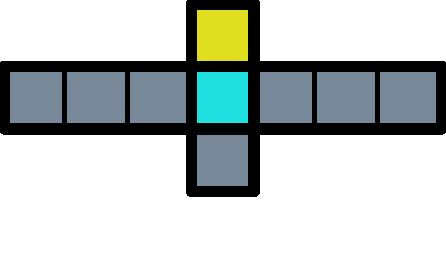
\includegraphics[width=0.9\textwidth]{./pictures/dominoes/proff-floating/scenario-1.pdf}
    \caption{}
    \label{floating:a}
  \end{subfigure}
  \begin{subfigure}[b]{0.15\textwidth}
    \centering
    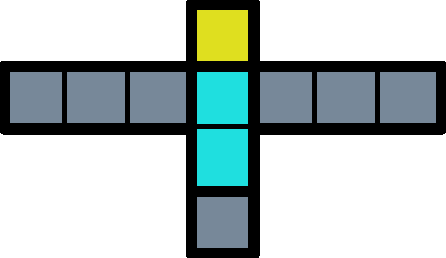
\includegraphics[width=0.9\textwidth]{./pictures/dominoes/proff-floating/scenario-2.pdf}
    \caption{}
    \label{floating:b}
  \end{subfigure}
  \begin{subfigure}[b]{0.15\textwidth}
    \centering
    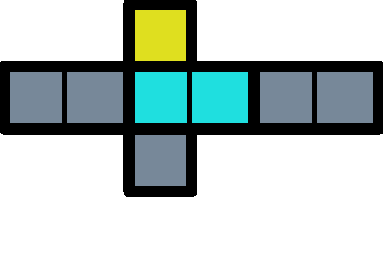
\includegraphics[width=0.9\textwidth]{./pictures/dominoes/proff-floating/scenario-3.pdf}
    \caption{}
    \label{floating:c}
  \end{subfigure}
  \caption{In yellow, the cell \( \cell[r+1][j]_{k-1} \), which is below row \( r \), is going to be cleared in the next turn.}
  \label{dom:drs}
\end{figure}

In scenario~\ref{floating:a}, there's no way to fill cell \( \cell[r][j]_{k-1} \), since there is no trajectory to place a domino there. In scenario~\ref{floating:b}, to place a domino that fills cells \( \cell[r][j-1]_{k-1} \) and \( \cell[r][j]_{k-1} \), at least one of \( \cell[r-1][j-1]_{k-1} \) or \( \cell[r-1][j]_{k-1} \) must be filled, leading to a filled cell under \( \cell_k \) after clearing row \( r \). Scenario~\ref{floating:c} follows analogously.

Thus, there is no way for this piece to be floating.
\end{proof}

Moreover, this lemma implies that in any constructible configuration, completely floating blocks--i.e., blocks whose lower corners do not touch any domino--cannot exist. This characterization also provides insight into the possible arrangements of holes and paths within the board. Before directly addressing the main problems, we will first examine two variations of the game: one where all dominoes are oriented vertically and another where all dominoes are oriented horizontally.

\subsection{Tetris with Vertical Dominoes}

Using the notation introduced earlier, the problem is denoted as $\textsc{Tetris-NoRotation}\lbrack \VD \rbrack$, considering both \clearing\ and \survival. The input consists of a sequence of vertical dominoes and an arbitrarily sized $n \times m$ board in a constructible configuration. The initial state function in this variation differs from the default orientation, as the pieces must be from the beginning in a vertical orientation.

\subsubsection{Constructible board configurations}

First we will to characterize the constructible boards with $\VD$ pieces without rotation by exploring the configuration starting from an empty board. 

Vertical dominoes consist of two vertical adjacent cells, so for an empty board any trajectory fixes the piece in the bottom row, filling $\cell[1][i]$ and $\cell[2][i]$ cells for any $1 \leq i \leq m$. The next domino can either go to an empty column or to the one before. Placing the first $m$ dominoes in unfilled columns clears the two lowest rows, and consequently the board. When a domino is placed in a non-empty column $i$, the $\cell[3][i]$ and $\cell[4][i]$ are filled, and so on, util a $\VD$ is placed in the last unfilled column. When this happens the two lowest rows are cleared and the process continues. 

So we can represent a reachable configuration of a given $n \times m$ board $B$ with a sequence of $m$ integers $(a_1, \dots, a_m)$, where

$$0 \leq a_i \leq \lceil \frac{n}{2} \rceil, \;\;\;   \forall i = 1,\dots, m$$

and $\exists i$ such that $a_i = 0$ (an empty column), with the following mapping: 

$$
\cell = \begin{cases}
   \text{filled}  & \text{if } i \leq  2a_j  \\
   \text{empty}   & \text{if } i >  2a_j
\end{cases}
$$

Each $a_i$ counts the number of vertical pieces placed in the column $i$. For example, in a $10 \times 6 $  board, the sequence $(1,2,0,4,2,3)$ defines the configuration in 
\ref{dom:vconf}.

\begin{figure}[ht]
  \centering
  \begin{subfigure}[b]{0.2\textwidth}
    \centering
    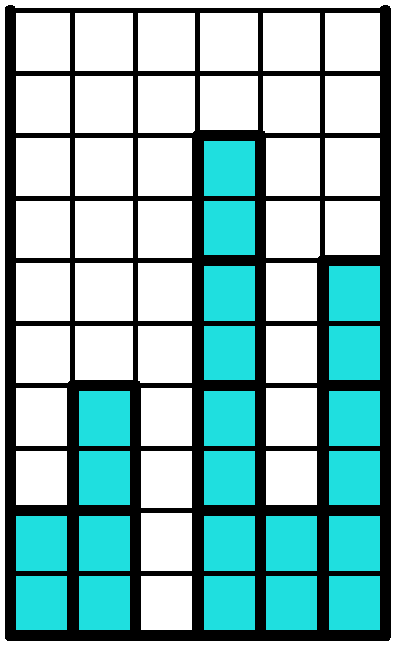
\includegraphics[width=0.9\textwidth]{pictures/dominoes/vertical_configuration.pdf}
    \caption{}
  \end{subfigure}
  \begin{subfigure}[b]{0.2\textwidth}
    \centering
    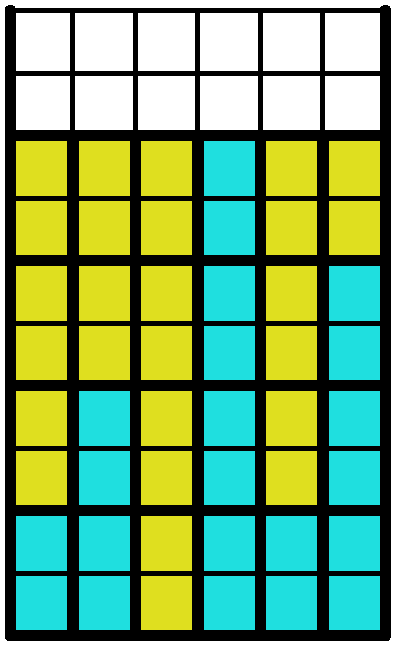
\includegraphics[width=0.9\textwidth]{pictures/dominoes/vertical_configuration_filled.pdf}
    \caption{}
  \end{subfigure}
    \caption{The $10 \times 6 $ board configuration represented by the sequence $(1,2,0,4,2,3)$, in yellow the 13 dominoes needed to clear the board.}
  \label{dom:vconf}
\end{figure}

\subsubsection{Cleaing}

In this decisional problem the input is a sequence of $k$ vertical dominoes and an $n \times m$ board with an initial configuration, that can be represented by the sequence $(a_1, \dots, a_m)$ as before. The question is: \emph{Is ther a way to clean the board after placing the $k$ pieces?}

\begin{theorem} 
$\textsc{Tetris-NoRotation}\lbrack \VD \rbrack $ \clearing\ is in \pp.
\label{dom:no-rot-vd}
\end{theorem}
\begin{proof}
    Let $B = (a_1, \dots, a_m) $ be the board representation and $k$ the length of the sequence of vertical dominoes. For every constructible board there is an empty column, so the strategy consists on placing each piece in an arbitrary empty column. 

    All the empty cells under the lowest empty row need to be filled to clean the board. Let $a_{\max}$ be the max in the board representation. Since we fill cells with dominoes, the number of dominoes $k_{\min}$ needed to clean the board is:
    $$ k_{\min} = \sum_{i = 1}^m \left( a_{\max} - a_i \right) $$

    If $k < k_{\min}$ we can't clear the board. If $k =  k_{\min}$ we can clear the board. And when $k > k_{\min}$, we can clean the board if after placing $k_{\min}$ dominoes the number of remaining pieces is a multiple of the board width, $k - k_{\min} \equiv 0 \mod m$. Since all the computations can be done in polyatomic time in respect of the input, the problem is in \pp.
\end{proof}

For boards with an even number of rows all pieces always fit inside the board. For an odd number of rows, dominoes could be placed in the top row with half of the domino inside the board and half outside. If we allow this, by changing the \emph{fix} function, the result would be the same since the same strategy works. The Figure~\ref{dom:vconf} shows, in yellow color, how the number of pieces needed to clean the board.

\subsubsection{Survival}

With the same input, the objective is to do not lose. The last proof provides a strategy to survive indefinitely. So for any number of pieces $k$ there is a way to avoid losing. Hence:
\begin{theorem} 
$\textsc{Tetris-NoRotation}\lbrack \VD \rbrack $ \survival\ is in \pp.
\end{theorem}


\subsection{Tetris with horizontal dominoes}

As before, the problem is $\textsc{Tetris-NoRotation}\lbrack \HD \rbrack$, considering both \clearing\ and \survival. Placing a horizontal domino fills two adjacent cells in one row or clears the row, meaning each domino placed can be tracked until the row is cleared. Thus, for any initial constructible configuration, the filled cells can be uniquely grouped into dominoes, allowing us to refer to dominoes instead of individual filled cells.

Additionally, in any constructible board, each row must contain an even number of filled cells. Consequently, when the board width is odd, no row can be cleared. In such cases, the board can only be cleared if it starts as an empty board with an empty sequence of pieces. From this point onward, we will assume that the board has an even number of columns. 

Let $B$ be a board with $m$ columns. We divide the board into $m/2$ \emph{buckets}, where each bucket consists of a pair of consecutive columns. Then:

\begin{lemma0}   
    Not placing a domino inside a bucket makes the row unclearable.
\end{lemma0}
\begin{proof}
    Let $r$ be a row containing some dominoes. When a domino is placed in a bucket it divides the row into two parts: the cells on the left side of the domino and the ones on the right. Both parts of even length, and containing an even number of filled cells.

    In the other case the two parts have an odd length but containing an eaven number of filled cells, making them impossible to clean
    since there's no way to add an odd number of cells by placing dominoes.
\end{proof}

For example, in the Figure~\ref{dom:buckets}, the second piece occupies the second and the third bucket, making the row un-clearable. 

\begin{figure}[h]
    \centering
    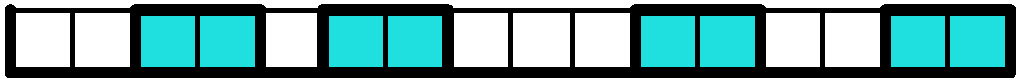
\includegraphics[width=0.2\textwidth]{./pictures/dominoes/buckets.pdf}
    \caption{A board with one partially filled row.}
    \label{dom:buckets} 
\end{figure}


We now can prove both clearing and survival problems.

\begin{theorem}
    $\textsc{Tetris-NoRotation}\lbrack \HD \rbrack $ \clearing\ is in \pp.
\end{theorem}
\begin{proof}


    The input is an $n \times m$ input board $B$, filled with a construable configuration, and sequence of $k$ dominoes $\HD$. If $m$ is odd then the board can't be cleared if $k > 0$ or the initial board isn't empty. 

    When $m$ is even we first need to check if the board is clearable. If there's only one row, checking that the row has been built by placing each piece inside a bucket determines if the row is clearable. When the board has more than one row the same happens. 

    We first group in pieces the filled cells of each row from the initial board. This can always be done because there's no way to clean \emph{"half"} piece. Then we check if each piece is placed inside a bucket. If some piece isn't placed inside a bucket the board can't be cleared. We can compute this in $\mathcal{O}(n\cdot m)$.

    Now the board can be represented with a sequence $(a_1, \dots, a_{m/2})$ of $m/2$ numbers each representing the number of dominoes placed in each bucket.

    $$
    \cell = \begin{cases}
        \text{filled}  & \text{if } i \leq  a_{2j}  \\
        \text{empty}   & \text{if } i >  a_{2j}
    \end{cases}
    $$

    With some $a_i = 0$. Let $a_{\max} = \max \{a_1, \dots a_{m/2}$ \} be the maximum of the sequence. The minimum number of pieces needed to clear the board is:

    $$ k_{\min} = \sum_{i = 1}^{m/2} (a_{\max} - a_i )$$

    If $k < k_{\min}$ the board can't be cleared. If $k = k_{\min}$ the board can be cleared. When $k > k_{\min}$ the board can be cleared if $ k - k_{\min} \equiv 0 \mod m / 2$, sine the remaining pieces have to leave the board empty by filling rows.
\end{proof}

\begin{figure}[ht]
  \centering
  \begin{subfigure}[b]{0.3\textwidth}
    \centering
    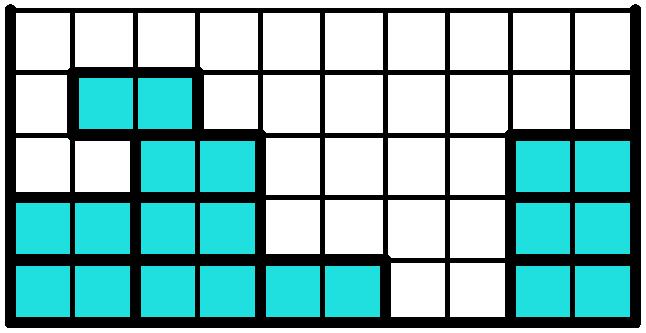
\includegraphics[width=0.9\textwidth]{pictures/dominoes/horitzonatl_configuration_1.pdf}
    \caption{}
  \end{subfigure}
  \begin{subfigure}[b]{0.3\textwidth}
    \centering
    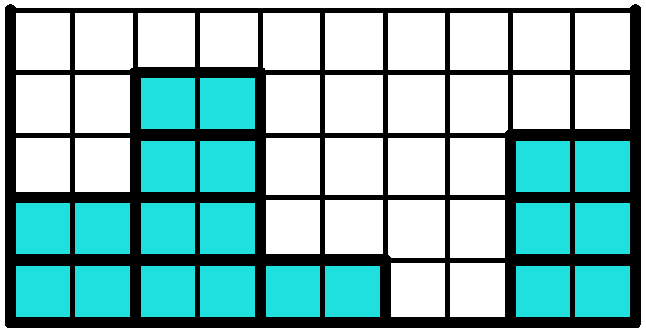
\includegraphics[width=0.9\textwidth]{pictures/dominoes/horitzonatl_configuration_2.pdf}
    \caption{}
  \end{subfigure}
  \begin{subfigure}[b]{0.3\textwidth}
    \centering
    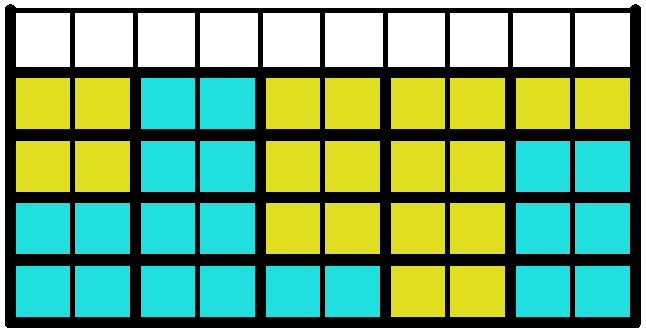
\includegraphics[width=0.9\textwidth]{pictures/dominoes/horitzonatl_configuration_3.pdf}
    \caption{}
  \end{subfigure}
  \caption{Some board configurations. In (a) the board can't be cleared because the topmost domino is placed between the first and the second bucket. In (b) the board is represented by the sequence $(2,4,1,0,3)$, it can be cleared. The minimum number of pieces to clean the board is 10, this pieces appear in yellow in (c).}
  \label{dom:horitzonatl_configuration}
\end{figure}

Figure~\ref{dom:horitzonatl_configuration} shows some examples of the above prof. Next follows the \survival. In this scenario the goal is to find a strategy to survive indefinitely, to survive indefinitely.  

\begin{theorem}
    $ \textsc{Tetris-NoRotation}\lbrack \HD \rbrack $ \survival\ is in \pp.
\end{theorem}
\begin{proof}
    
If a given board \( B \) contains a clearable row, we can survive indefinitely by first clearing this row and then continuing to place pieces to refill the topmost row. If no such row exists---for instance, on a board with odd width---there exists a maximum number \( k_{\max} \) of dominoes that can be placed before a loss becomes inevitable. Thus, if the input length \( k \) is less than or equal to \( k_{\max} \), survival is possible; otherwise, it is not. The following procedure checks if any row can be cleared and, if not, computes \( k_{\max} \).

Horizontal dominoes fit naturally in a row, so maximizing the number of dominoes placed on the board \( B \) requires maximizing their placement in each row. To avoid blocking further placements, the board is filled from the bottom to the top. Within a row, a \emph{hole} is defined as a set of contiguous empty cells bounded by filled cells or the board's edges. 

% More formally, for row \( r \), a \emph{hole} is a segment:
%
% \[h^r_{j_1,j_2} = \{\cell[r][j_1], \cell[r][j_1+1], \dots, \cell[r][j_2]\}\]
%
% where all cells in \( h \) are empty, and the boundary cells \( \cell[r][j_1-1] \) and \( \cell[r][j_2+1] \) are either filled or lie outside the board.

To maximize the number of dominoes in the board, each row's holes must be filled as completely as possible. This reduces the problem of filling the entire board to the simpler task of optimally filling individual row holes. By systematically filling holes from the bottom-most row upwards, we ensure the greatest number of dominoes are placed without causing unresolvable blocking and ensure that each hole is above a maximally filled row. 

Let \( h = \{\cell[r][j_1], \cell[r][j_1+1], \dots, \cell[r][j_2]\} \) represent a hole in row \( r \) spanning columns \( j_1 \) to \( j_2 \). All cells in \( h \) are empty, and the boundary cells \( \cell[r][j_1-1] \) and \( \cell[r][j_2+1] \) are either filled or lie outside the board. To place a domino inside the hole, there must exist a trajectory from the top of the board to \( h \), making only reachable holes relevant for consideration.

Using Lemma~\ref{lem:floating} a hole must take one of the following shapes:

\begin{figure}[ht]
  \centering
  \begin{subfigure}[b]{0.24\textwidth}
    \centering
    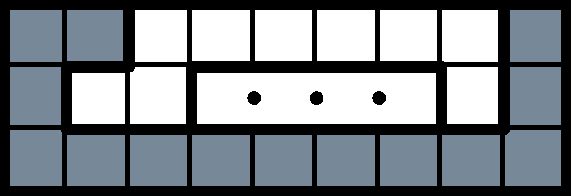
\includegraphics[width=0.9\textwidth]{pictures/dominoes/simple-hole-1.pdf}
    \caption{}
    \label{dom:hole-a}
  \end{subfigure}
  \begin{subfigure}[b]{0.24\textwidth}
    \centering
    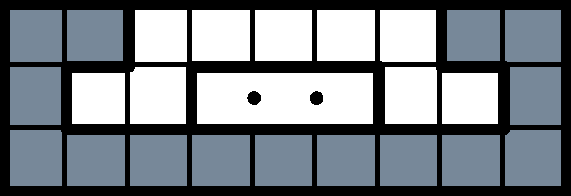
\includegraphics[width=0.9\textwidth]{pictures/dominoes/simple-hole-2.pdf}
    \caption{}
    \label{dom:hole-b}
  \end{subfigure}
  \begin{subfigure}[b]{0.24\textwidth}
    \centering
    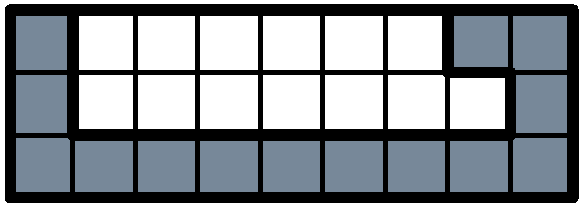
\includegraphics[width=0.9\textwidth]{pictures/dominoes/simple-hole-3.pdf}
    \caption{}
    \label{dom:hole-c}
  \end{subfigure}
  \begin{subfigure}[b]{0.24\textwidth}
    \centering
    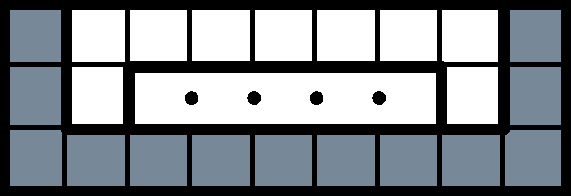
\includegraphics[width=0.9\textwidth]{pictures/dominoes/simple-hole-4.pdf}
    \caption{}
    \label{dom:hole-d}
  \end{subfigure}
  \label{dom:holes}
\end{figure}

Let \( l = j_2 - j_1 + 1 \) denote the length of the hole \( h \). The maximum number of dominoes that can be placed in holes of type \ref{dom:hole-a} and \ref{dom:hole-c} is \( \lfloor l / 2 \rfloor \) for $l > 2 $, completely filling the hole if \( l \) is even. For a hole of type \ref{dom:hole-b}, the same rule applies for \( l > 4 \). For $l = 4$ only one domino can be placed, as shown in Figure~\ref{dom:hole-4}.

\begin{figure}[h]
    \centering
    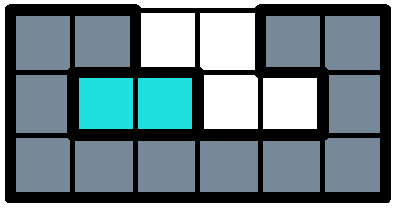
\includegraphics[width=0.18\textwidth]{./pictures/dominoes/hole-4.pdf}
    \caption{A type-\ref{dom:hole-b} hole of length 4.}
    \label{dom:hole-4} 
\end{figure}

Finally, the algorithm to decide the problem would look like:
\begin{algorithmic}[1]
    \Function{Tetris-NoRotation[$\HD$]}{$B,k$} \Comment{a board $B$ and $k$ dominos}
    \State $k_{\max}\gets 0$ \Comment{tracks if each hole of a row is fully filled}

    \For{row $r = 1, \dots, n$}
    \State $\text{full} \gets \text{True}$
      \For{hole $h$ in $r$}
        \State $k = \text{MaxDominoes}(h)$ \Comment{the $k$ dominoes that can be maximally placed in $h$}
        \If{$2 \cdot k_r \neq \text{length}(h)$}
          \State $\text{full} \gets \text{False}$
        \EndIf
        \State $k_{\max} = k_{\max} + k$
      \EndFor

      \If{ $\text{full}$}
        \State \textbf{return} $\text{True}$ \Comment{surviving indefinitely}
    \EndIf
\EndFor

\State \textbf{return} $k \leq k_{\max}$
\EndFunction
\end{algorithmic}

The cost of the algorithm is $\mathcal{O}(n \cdot m)$, since looping throught the holes has cost $\mathcal{O}(m)$ and filling the hole maximally has constant cost when the hole shape is known.

\end{proof}


\subsection{Tetris Survival Without Rotation}

The problem $\textsc{Tetris-NoRotation}\lbrack \VD \rbrack $ \survival\ can be formulated as follows: \emph{Given an arbitrarily sized board with an constructible initial configuration and a sequence of \( k \) dominoes, is there a way to play all the pieces while avoiding losing?} As pointed out in \cite{TT}, if there exists a strategy to clear a single row, it is possible to survive indefinitely by employing the following piece-placement strategy:

\begin{enumerate}
    \item Rotate the piece to be vertical. 
    \item Place the piece in any column with the two top cells empty.
\end{enumerate}

To solve the problem, we must demonstrate that, when the top row is not empty, deciding whether any row can be cleared is in \pp. 

\vspace{10px}

We will address the problem in two parts: determining the conditions under which the first row can be cleared and identifying the conditions for clearing any subsequent row. Let's first see a lemma that will help in both proofs.

\begin{lemma0}
Let $B$ be an $n \times m$ board in a constructible configuration and $p$ a reachable path. Determining whether a domino can be fixed in any position of the path, possibly placing additional dominoes below, it can be computed in \( O(??) \).
\end{lemma0}

\begin{proof}
  Let $p = \{ c_1, \dots, c_k \} $ be the path. Let $c_{k-1}, c_{k} \in p$ be the target position to fix the domino. Let's first consider the case that

  si l'ehm de colocar verical podem passart tres escenarios respecte les peces de sota. 

  - buida buida buida -> fotali horzontals fins que se pugi
  - pelna buida buida -> fotali horzontals fins que se pugi
  - buida buida pelna -> fotali horzontals fins que se pugi
  - pelna buida pelna -> fes la pregunta a sota

  cheeeek
\end{proof}


\begin{lemma0}
For any $n \times m$ board, deciding whether the top row can be cleared is in \pp.
\end{lemma0}
\begin{proof}
\end{proof}

\begin{lemma0}
For any $n \times m$ board, deciding if any row, except the first one, can be cleared is in \pp.
\end{lemma0}

\begin{proof}
  Let $r < m$ be the row to be checked. To fill completely the row all the holes need to be fully filled. Let $h = \{ \cell[r][j_1], \dots, \cell[r][j_2]\}$ a hole in row $r$ from column $j1$ to column $j_2$.  

\end{proof}
